\documentclass[titlepage,a4paper]{jsarticle}
\usepackage{../../../sty/import}% 各種パッケージインポート
\usepackage{../../../sty/title}% タイトルページの変更

%% タイトルページの変数
% レポートタイトル
\title{WebAPIを使用したスマートフォンアプリ}
% 提出日
\expdate{\today}
% 12/27 17:00まで
% 科目名
\subject{情報システム工学演習}
% 分野
\class{情報経営システム工学分野}
% 学年
\grade{B3}
% 学籍番号
\mynumber{24336488}
% 記述者
\author{本間三暉}

\begin{document}
% titleページ作成
\maketitle

\section{目的}
% このアンケートシステム(DataBase,Repository,Domain,Servlet,JSP+WebAPI+スマートフォンアプリ)の目的を記載すること。
本レポートの目的は,授業の一環として個人で開発したアンケートシステムについて,その企画・設計・実装の全過程を詳細に記録し,そこから得られた技術的知見や自己成長の成果を明確化することである.
本システムは,ユーザーが簡便かつ効率的にアンケートを作成・配布・集計できることを目指し,実用性と操作性を重視して設計された.
開発を通じて,Webアプリケーション開発の基礎知識やフレームワークの使用方法だけでなく,データベース設計やセキュリティ対策の重要性についても実践的に学習した.

本レポートでは,これらのプロジェクト全体を振り返り,成功した点や改善すべき点を整理し,次回の開発に生かすための具体的な指針を提示する.
特に,データの管理手法,ユーザーエクスペリエンスの向上,および個人開発における効率的な問題解決のアプローチについて考察する.
この振り返りを通じて,単なる技術習得にとどまらず,今後のより高度な開発への応用力を高めることを目指す.
\section{原理と構成}
% このシステムの構成を図で示し、どのような仕組みで動作するかを説明してください。
% (※図は手書きでもかまいません)
\subsection{Webアプリケーション}
図\ref{web}にWebアプリケーションのシステム構成を示す.
\begin{figure}[H]
  \centering
  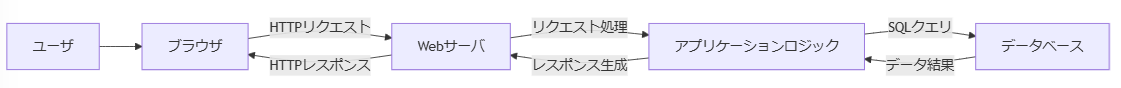
\includegraphics[width=0.8\textwidth]{img/genri/web.png}
  \caption{Webアプリケーションのシステム構成}
  \label{web}
\end{figure}
Webアプリケーションは,クライアント(ユーザが使用するブラウザ)とサーバが通信を行い,データの取得や操作を実現するシステムである.
ユーザがブラウザを通じて操作すると,ブラウザはHTTPリクエストをサーバに送信し,サーバはデータベースと連携してリクエストに応じたデータを処理し,HTMLやJSON形式でレスポンスを返す.
この一連の流れは以下のように進行する.
\subsubsection{クライアントからのリクエスト送信}
ユーザがブラウザでボタンをクリックするなどの操作を行うと,JavaScriptが動作してサーバにリクエストを送信する.
このリクエストは「GET」や「POST」などのHTTPメソッドを使用しており,送信データやクエリが含まれる.

\subsubsection{サーバ側での処理}
サーバはリクエストを受け取ると,対応するプログラム(アプリケーションロジック)を実行する.
ここで,データベースに対してSQLクエリを発行し,必要なデータを取得または更新する.

\subsubsection{レスポンスの送信}
サーバは処理結果をHTMLやJSON形式に変換し,HTTPレスポンスとしてブラウザに送信する.

\subsubsection{ブラウザによる表示}
ブラウザは受信したレスポンスを元に画面を更新する.
この過程では,JavaScriptが動的に表示内容を変更することも可能である.\\

このように,Webアプリケーションはブラウザを介して動作し,インターネット接続を必要とする.
主にHTMLやJSON形式を使用してデータをやり取りするため,デザインや表示の柔軟性に優れている.

\subsection{スマートフォンアプリ}
図\ref{app}にスマートフォンアプリのシステム構成を示す.
\begin{figure}[H]
  \centering
  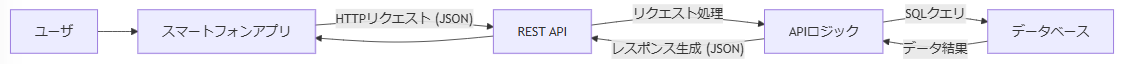
\includegraphics[width=0.8\textwidth]{img/genri/app.png}
  \caption{スマートフォンアプリのシステム構成}
  \label{app}
\end{figure}
スマートフォンアプリは,ネイティブ環境で動作するアプリケーションであり,Web APIを利用してサーバとの通信を行う.
スマートフォンアプリは,Webアプリケーションと同様にサーバとデータをやり取りするが,データの送受信には主にJSON形式が用いられる.
また,通信の効率化やパフォーマンス向上のためにREST APIが利用される.

\subsubsection{ユーザ操作によるリクエスト送信}
ユーザがアプリ内のボタンを押すなどの操作を行うと,アプリがWeb APIにHTTPリクエストを送信する.
このリクエストには,リソースを特定するための情報(例: 商品IDやユーザデータ)が含まれる.

\subsubsection{Web APIによる処理}
APIサーバはリクエストを受け取ると,リソースの取得,作成,更新,削除を実行するためにサーバ内のビジネスロジックを実行する.
さらに,必要に応じてデータベースと通信してデータを取得または操作する.

\subsubsection{レスポンスの受信}
APIサーバは処理結果をJSON形式に変換し,スマートフォンアプリに返送する.

\subsubsection{アプリ内でのデータ表示}
アプリは受信したデータをもとに画面を更新し,ユーザに視覚的に情報を提供する.
スマートフォンアプリではネイティブコードを利用するため,リッチなユーザインターフェースを構築できる.\\

スマートフォンアプリは,Web APIを通じた効率的な通信と,オフラインモードなどの高度な機能をサポートしている点が特徴的である.
また,データのやり取りには主にJSON形式が用いられ,軽量かつ扱いやすい.

\section{動作確認結果}
% スマートフォン画面のキャプチャ画像などを使って、作成したシステムが正常に動作していることを示してください。
\subsection{Webアプリケーション}
Webアプリケーションの動作結果を図\ref{webfig}に示す.

\begin{figure}[H]
  \centering
  \begin{minipage}[t]{0.45\textwidth}
    \centering
    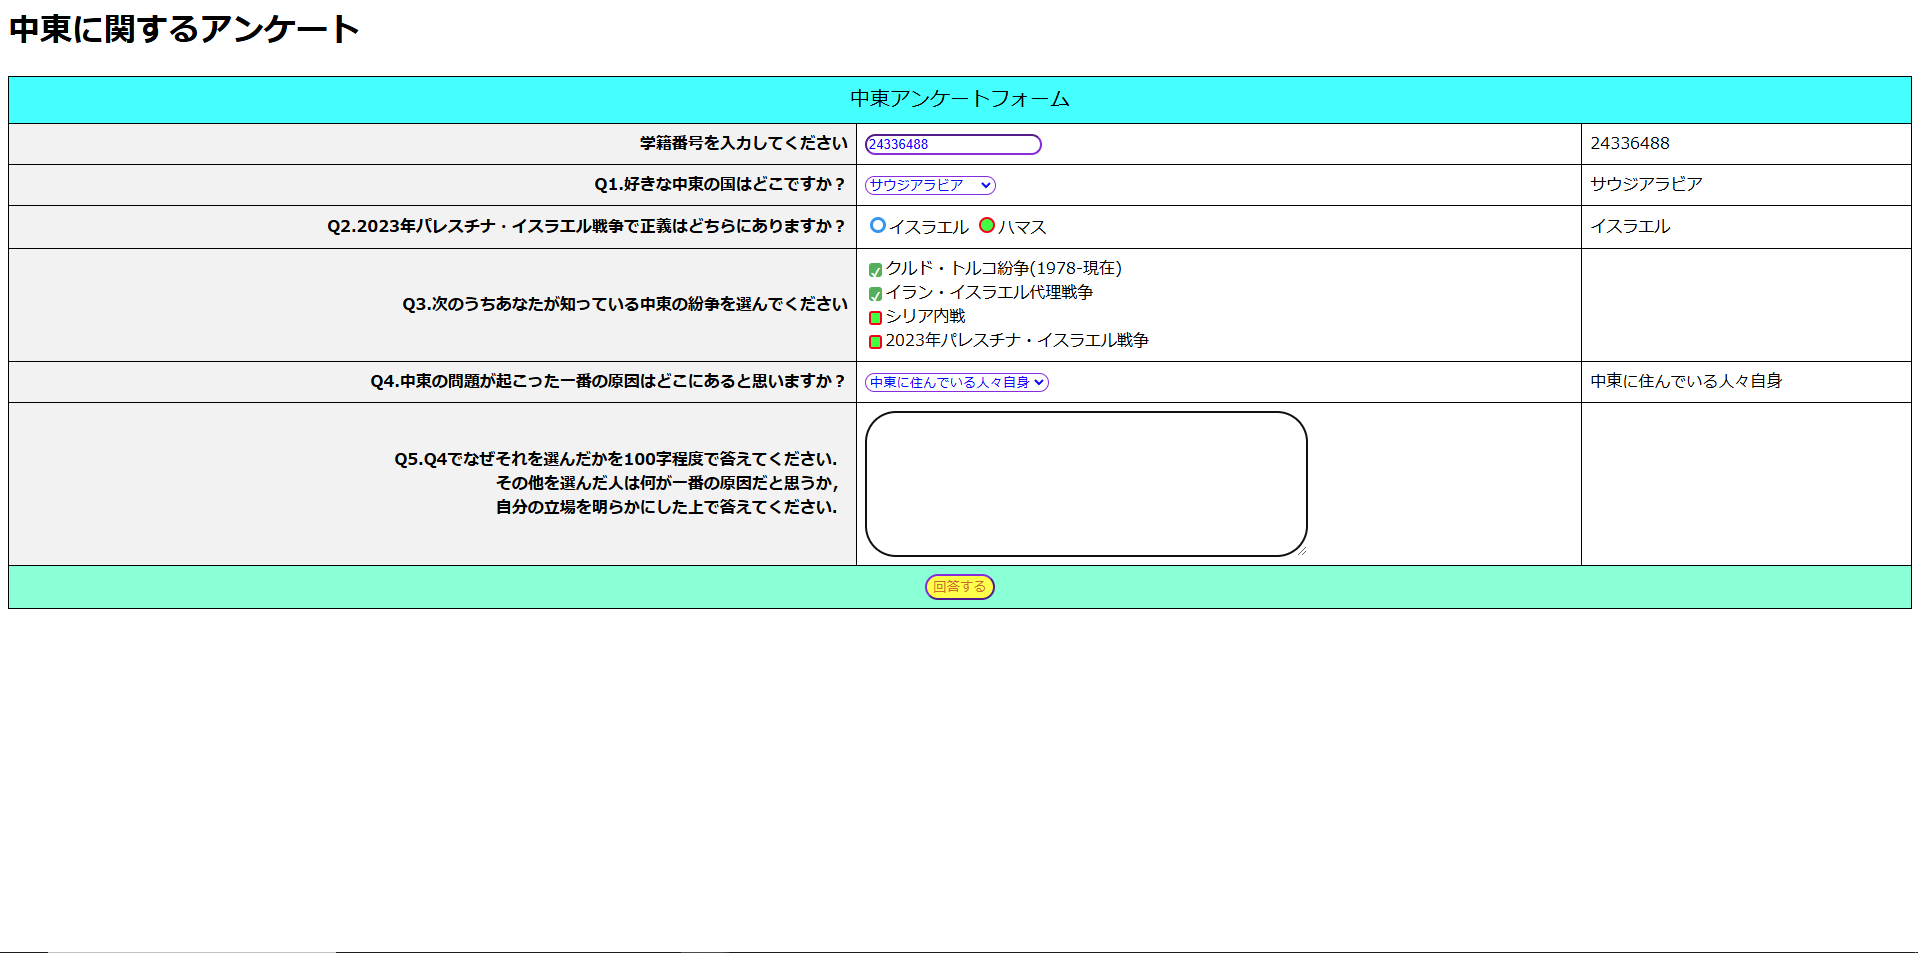
\includegraphics[width=\textwidth]{img/move/web1.png}  % 画像A
    \subcaption{Q1.html}
  \end{minipage}
  \hfill
  \begin{minipage}[t]{0.45\textwidth}
    \centering
    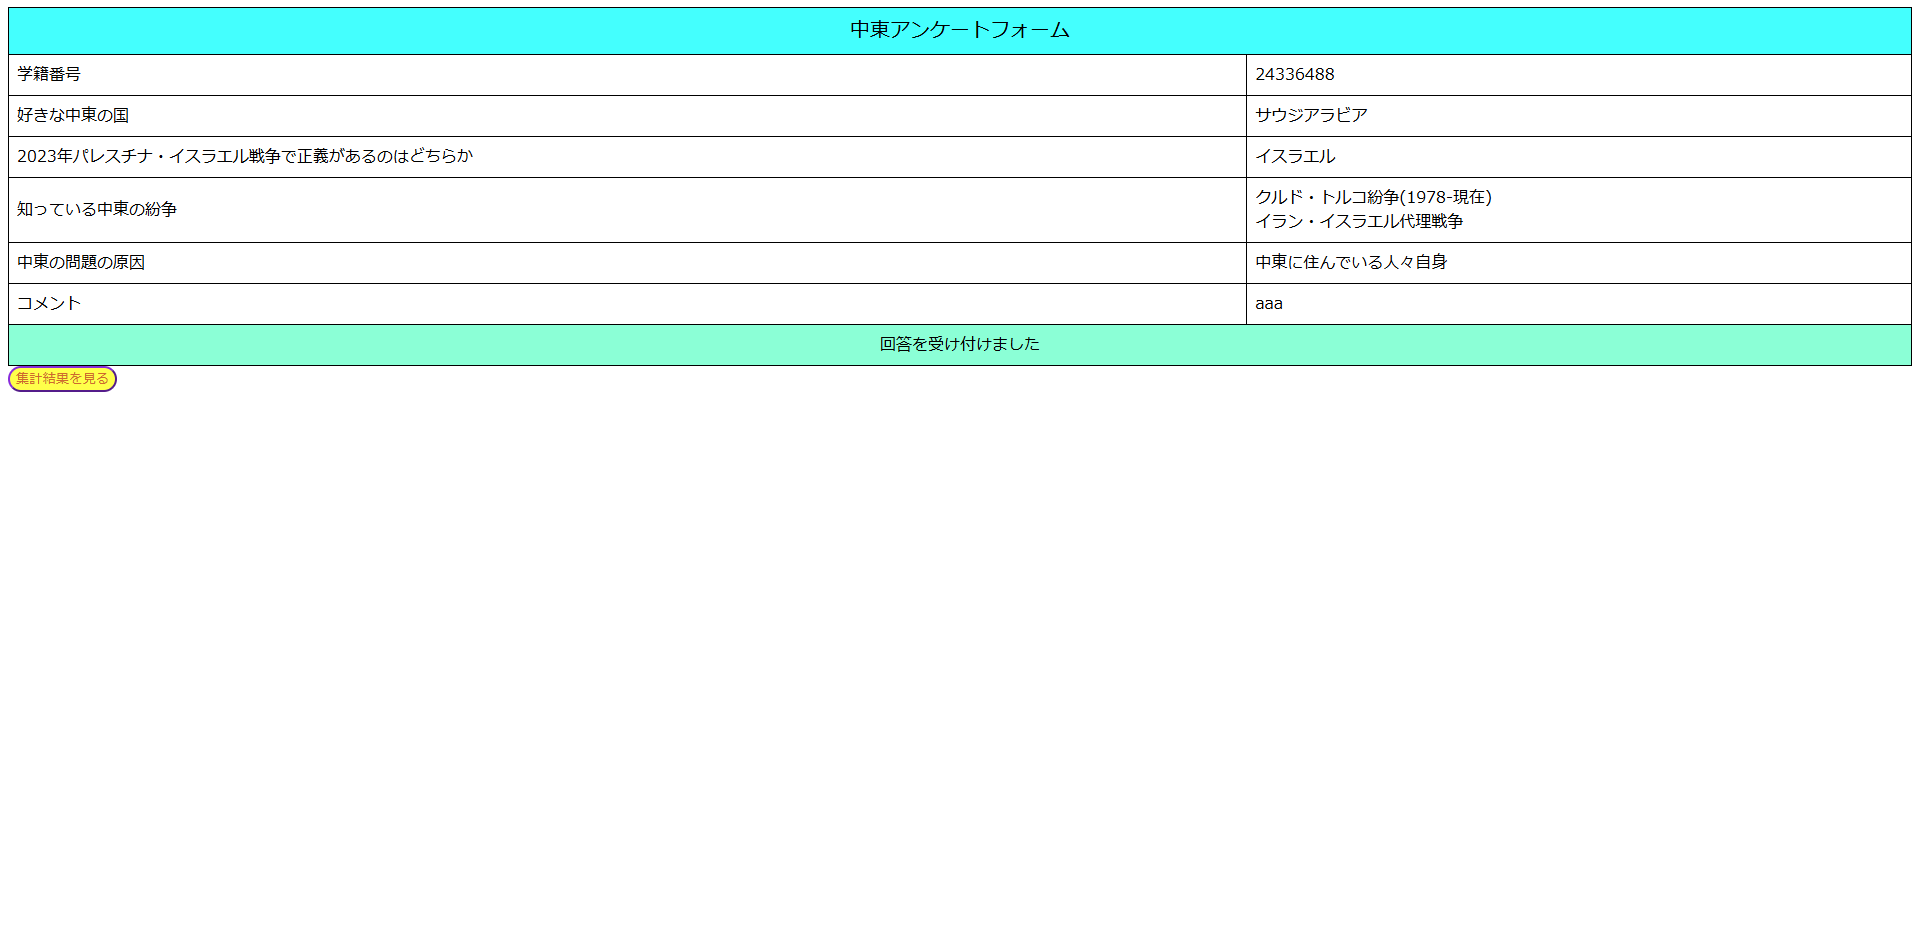
\includegraphics[width=\textwidth]{img/move/web2.png}  % 画像B
    \subcaption{Q1.jsp}
  \end{minipage}

  \vspace{0.5cm}  % 画像間の縦のスペース

  \begin{minipage}[t]{0.45\textwidth}
    \centering
    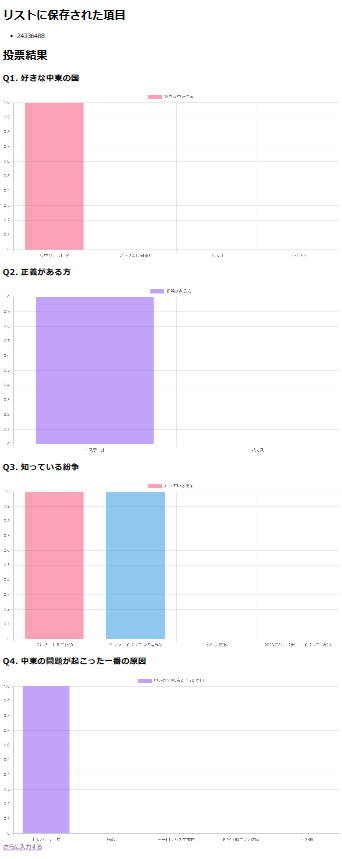
\includegraphics[height=0.5\textheight]{img/move/web3.png}  % 画像C(縦長)
    \subcaption{ResultServlet.jsp}
  \end{minipage}
  \caption{Webアプリケーションの動作結果}
  \label{webfig}
\end{figure}
しっかり値が入力され,その値を表示できていることがわかる.
\subsection{スマートフォンアプリ}
スマートフォンアプリの動作結果を図\ref{appfig}に示す.
\begin{figure}[H]
  \centering
  % 上段 (A, B)
  \begin{minipage}[t]{0.40\textwidth}
    \centering
    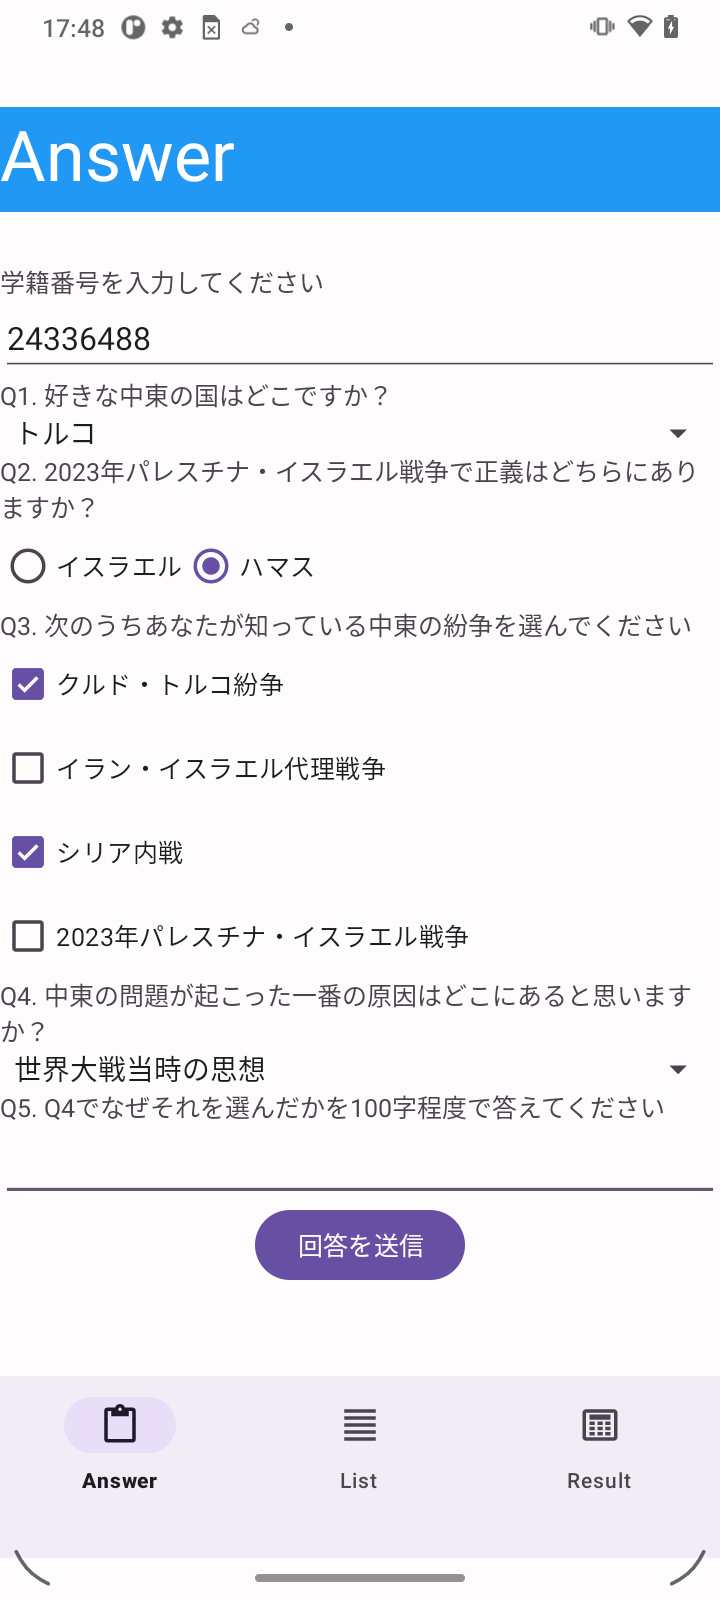
\includegraphics[height=0.35\textheight]{img/move/app1.png}
    \subcaption{Answer}
  \end{minipage}
  \hfill
  \begin{minipage}[t]{0.40\textwidth}
    \centering
    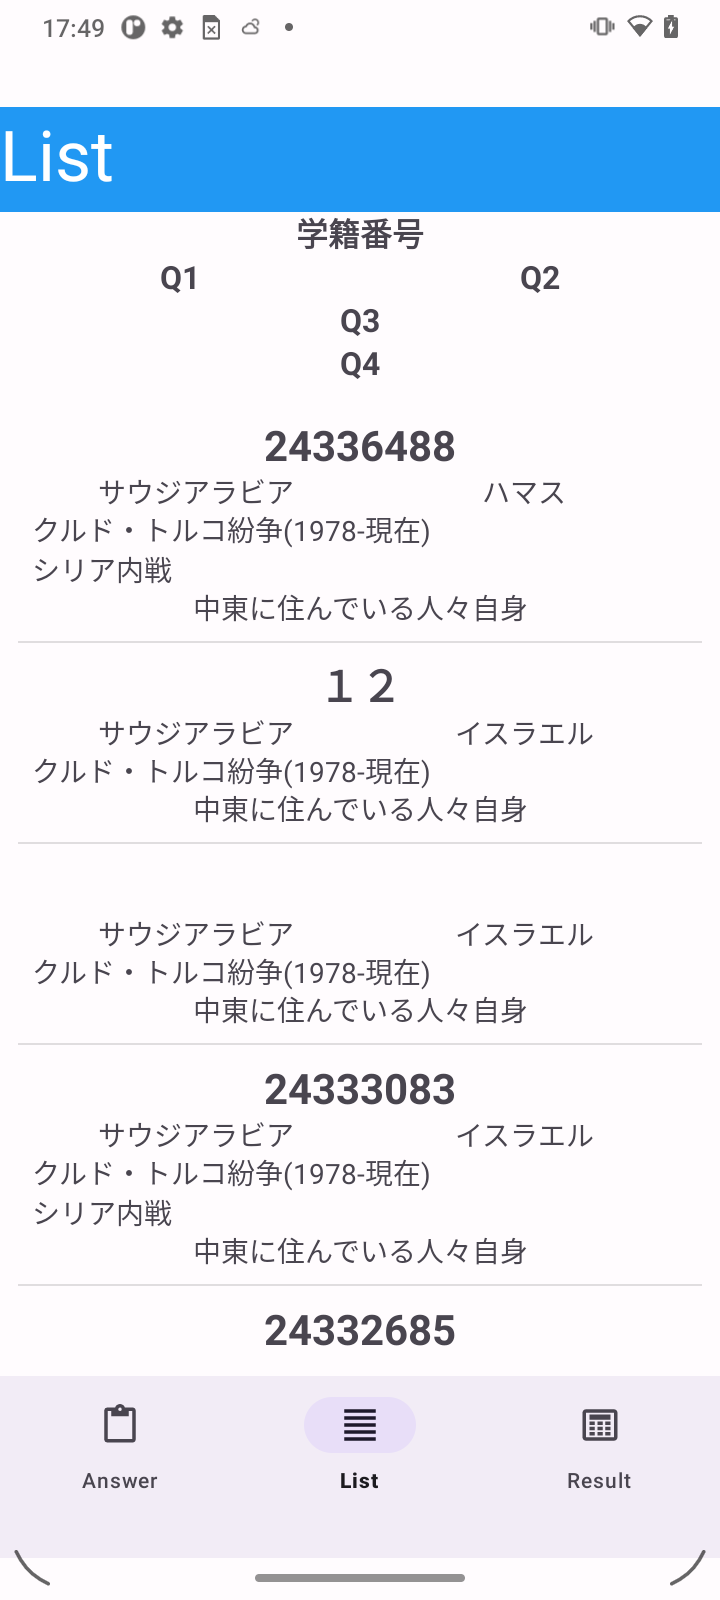
\includegraphics[height=0.35\textheight]{img/move/app2.png}
    \subcaption{List}
  \end{minipage}

  \vspace{0.5cm} % 上段と下段の間のスペース

  % 下段 (C, D, F)
  \begin{minipage}[t]{0.3\textwidth}
    \centering
    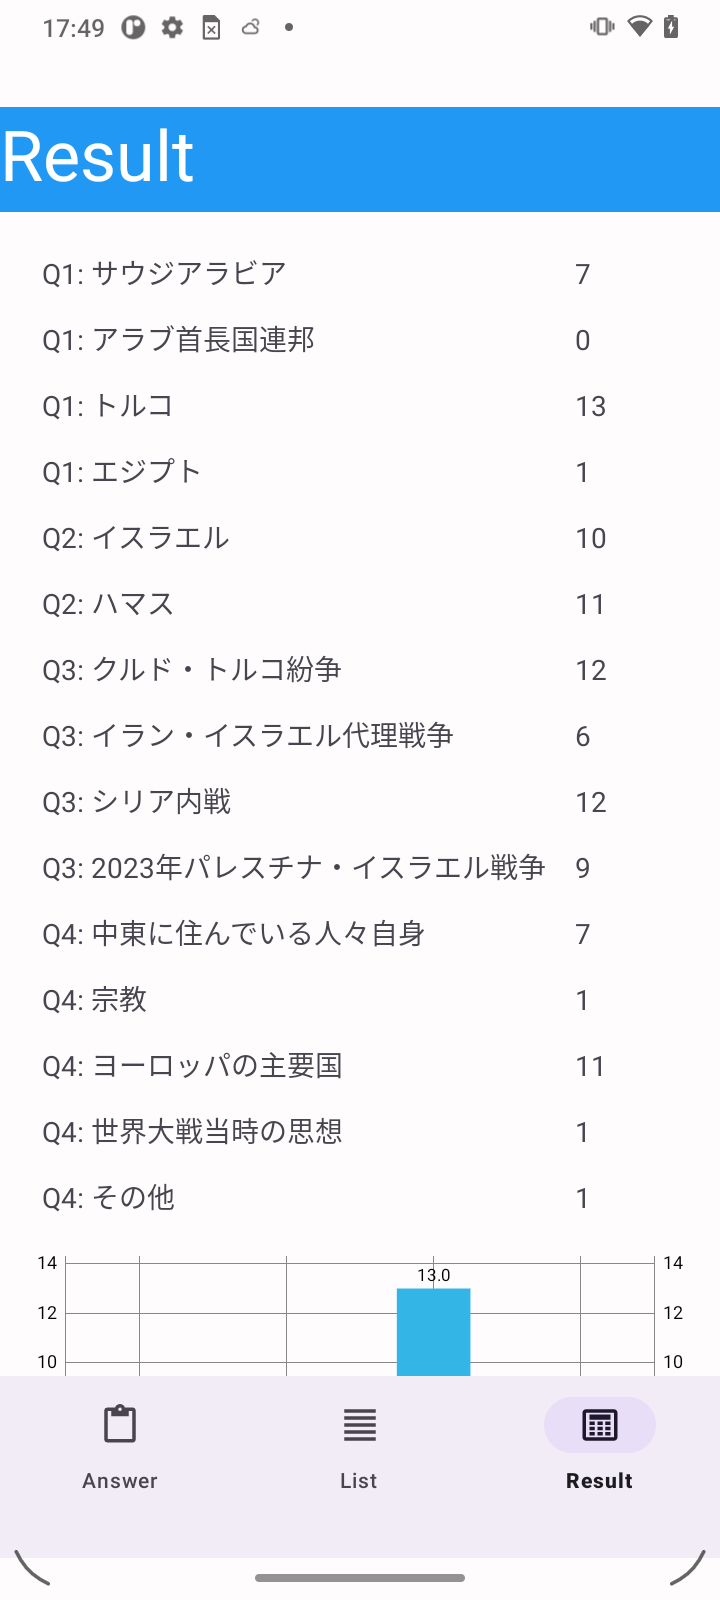
\includegraphics[height=0.4\textheight]{img/move/app3.png}
    \subcaption{Result1}
  \end{minipage}
  \hfill
  \begin{minipage}[t]{0.3\textwidth}
    \centering
    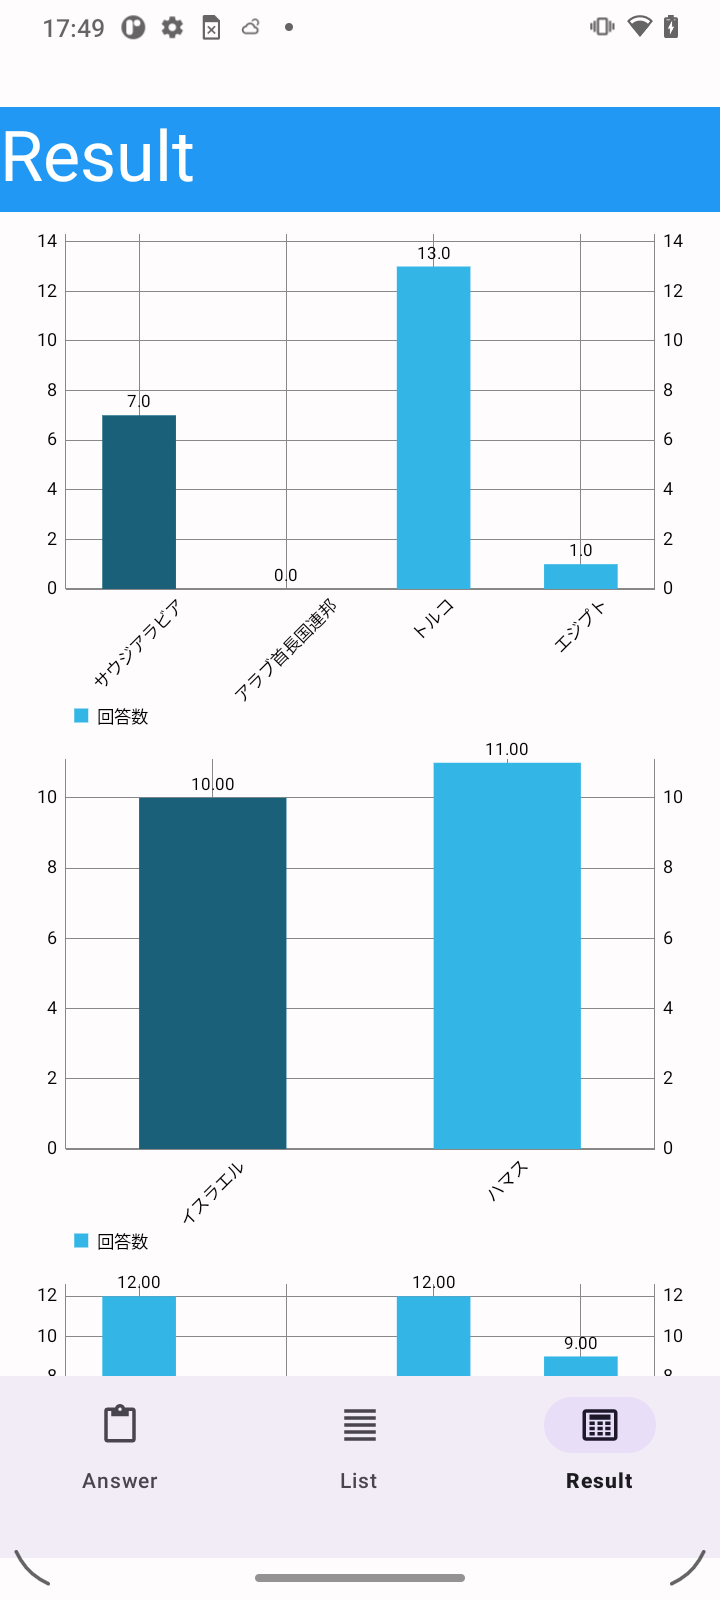
\includegraphics[height=0.4\textheight]{img/move/app4.png}
    \subcaption{Result2}
  \end{minipage}
  \hfill
  \begin{minipage}[t]{0.3\textwidth}
    \centering
    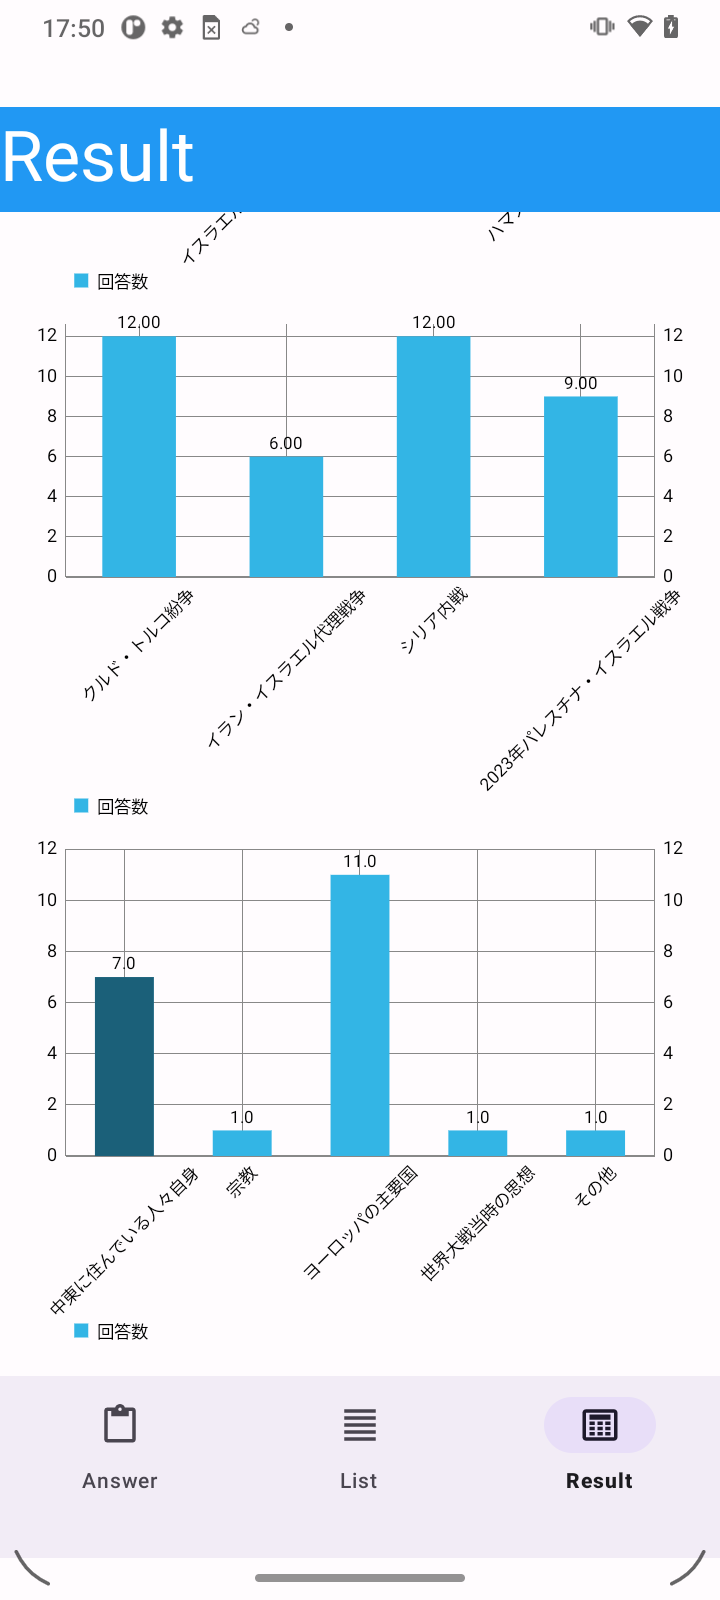
\includegraphics[height=0.4\textheight]{img/move/app5.png}
    \subcaption{Result3}
  \end{minipage}
  \caption{スマートフォンアプリの動作結果}
  \label{appfig}
\end{figure}
このように,データの入力,リスト表示,グラフ形式での表示に対応しており,動作として十分なものであると言える.

\section{考察}
%   以下について考察してください。
% ①    このシステムの長所
% ②    このシステムのSecurity
\subsection{このシステムの長所}
このシステムは概ねMVCであると考えられる.
MVCのような3層アーキテクチャは,アプリケーションをプレゼンテーション層(ユーザインターフェース層),ビジネスロジック層(アプリケーション層),データアクセス層の3つに分けて構成する設計手法である.
この構成は,それぞれの層に異なる責務を持たせることで,開発や保守の効率性を高めることを目的としている.

この設計の利点の一つは,関心の分離が明確である点である.
各層が異なる役割を持つため,コードの理解や修正が容易となり,システム全体の複雑さを軽減できる.
また,各層が独立していることで,特定の層を他のプロジェクトや異なる文脈で再利用することも可能であり,再利用性が向上する.

さらに,各層ごとにテストを実施できるため,機能の検証が効率的に行える点も大きな利点である.
例えば,ビジネスロジック層のロジックを個別にテストすることで,問題箇所を特定しやすくなる.
また,ユーザインターフェースの変更が必要な場合でも,プレゼンテーション層だけを修正すればよいため,他の層への影響を最小限に抑えられる.
この柔軟性は,仕様変更や機能追加が頻繁に発生する開発プロジェクトにおいて特に重要である.

加えて,各層が明確に分かれていることで,異なるチームやメンバーが同時並行で作業を進めやすくなり,チーム開発の効率化にも寄与する.
このような利点により,3層アーキテクチャは堅牢で保守性の高いアプリケーション開発に適した構成とされている.

\subsection{このシステムのSecurity}
% 「’); delete from testAnswer; --」ではエラーが出ない.「<script>alert(document.cookie);</script>」ではアラートが出てしまう.cookieは存在するか怪しい.
Webサイトを攻撃する方法として以下のものが挙げられる.
\begin{enumerate}
  \item SQLインジェクション (SQL Injection)
  \item クロスサイトスクリプティング (XSS: Cross-Site Scripting)
  \item クロスサイトリクエストフォージェリ (CSRF: Cross-Site Request Forgery)
  \item DDoS攻撃 (Distributed Denial of Service)
  \item ディレクトリトラバーサル (Directory Traversal)
  \item セッションハイジャック (Session Hijacking)
  \item ブルートフォース攻撃 (Brute Force Attack)
  \item ゼロデイ攻撃 (Zero-Day Attack)
  \item フィッシング (Phishing)
  \item サーバーサイドリクエストフォージェリ (SSRF: Server-Side Request Forgery)
\end{enumerate}

今回の授業では,システム自体とデータベースを作成することが目的であるので,``SQLインジェクション'',``クロスサイトスクリプティング'',``セッションハイジャック''などについて考察する.
\subsubsection{SQLインジェクション}
SQLインジェクションとは,悪意のあるSQLクエリを入力してデータベースを操作し,データの取得,改ざん,削除を試みる攻撃のことである.
今回は\textbf{'); delete from testAnswer; --}と\textbf{"); delete from testAnswer; --}というコマンドを入力して攻撃を試みた.
今回作ったWebページに攻撃を仕掛けた結果をそれぞれ図\ref{SQL_Injection1},\ref{SQL_Injection2}に示す.

\begin{figure}[H]
  \centering
  % 左側の画像
  \begin{minipage}[t]{0.45\textwidth}
    \centering
    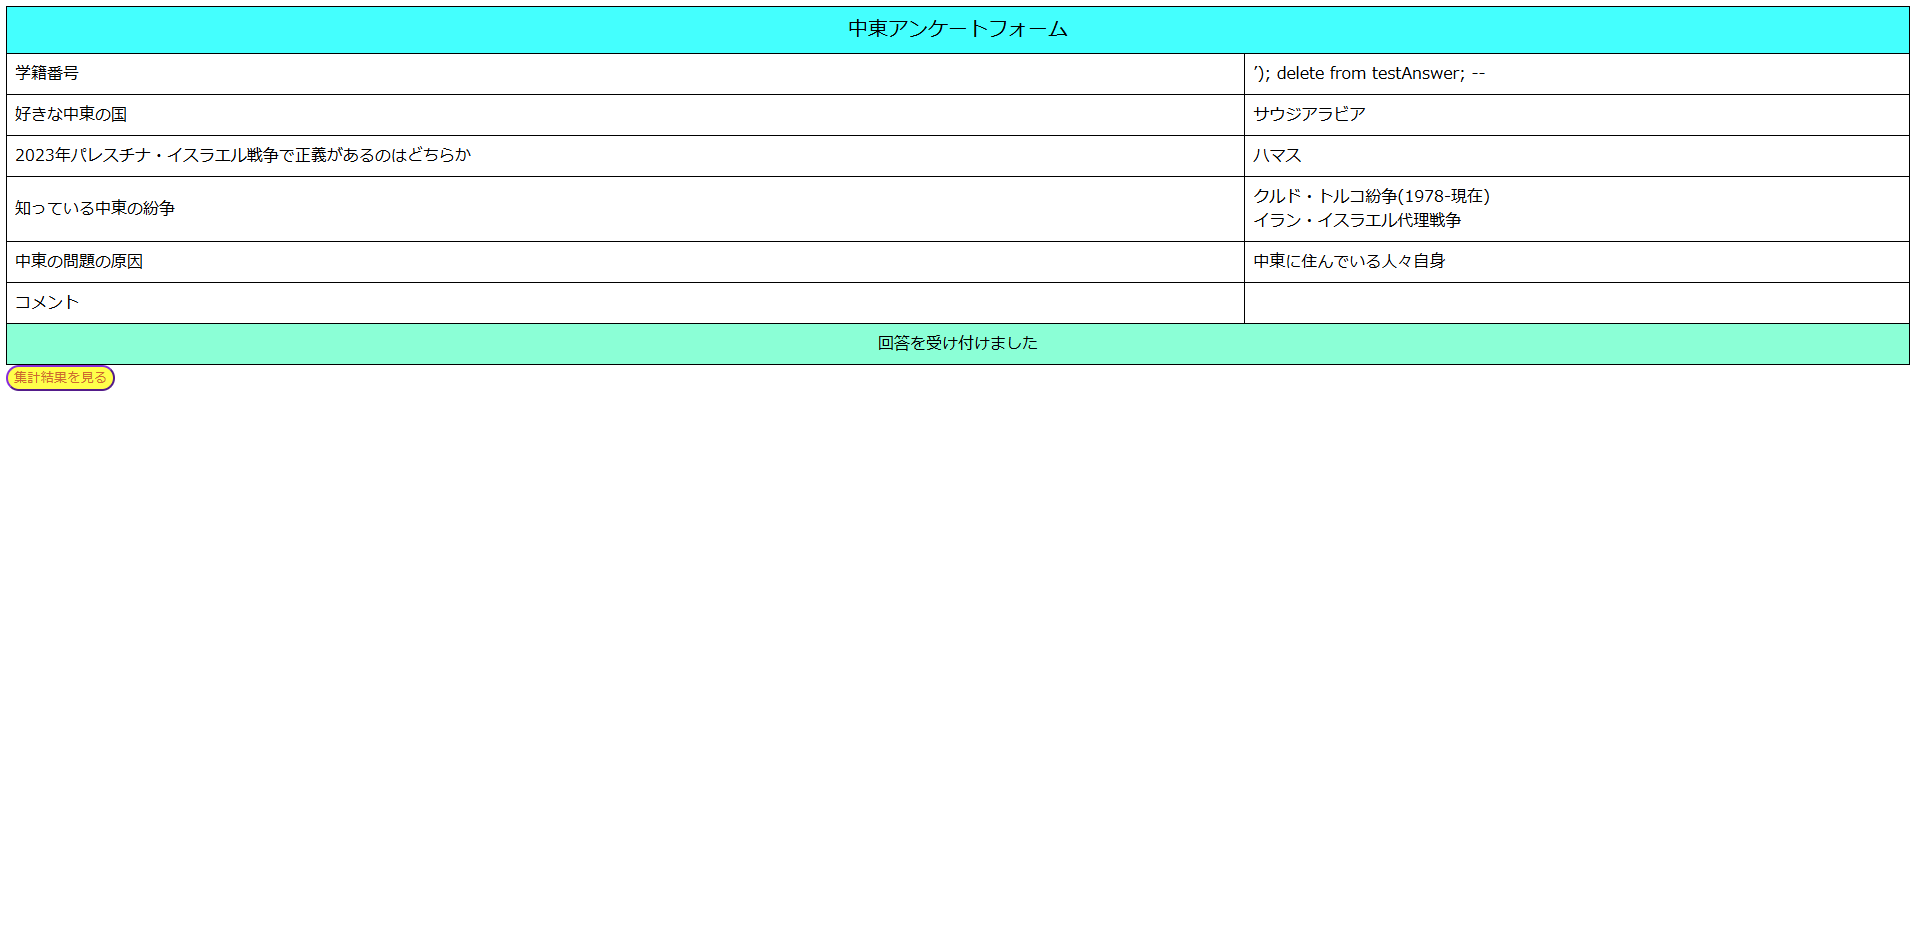
\includegraphics[width=\textwidth]{img/security/before_1.png}
    \subcaption{入力画面}
  \end{minipage}
  \hfill % 隙間を作る
  % 右側の画像
  \begin{minipage}[t]{0.45\textwidth}
    \centering
    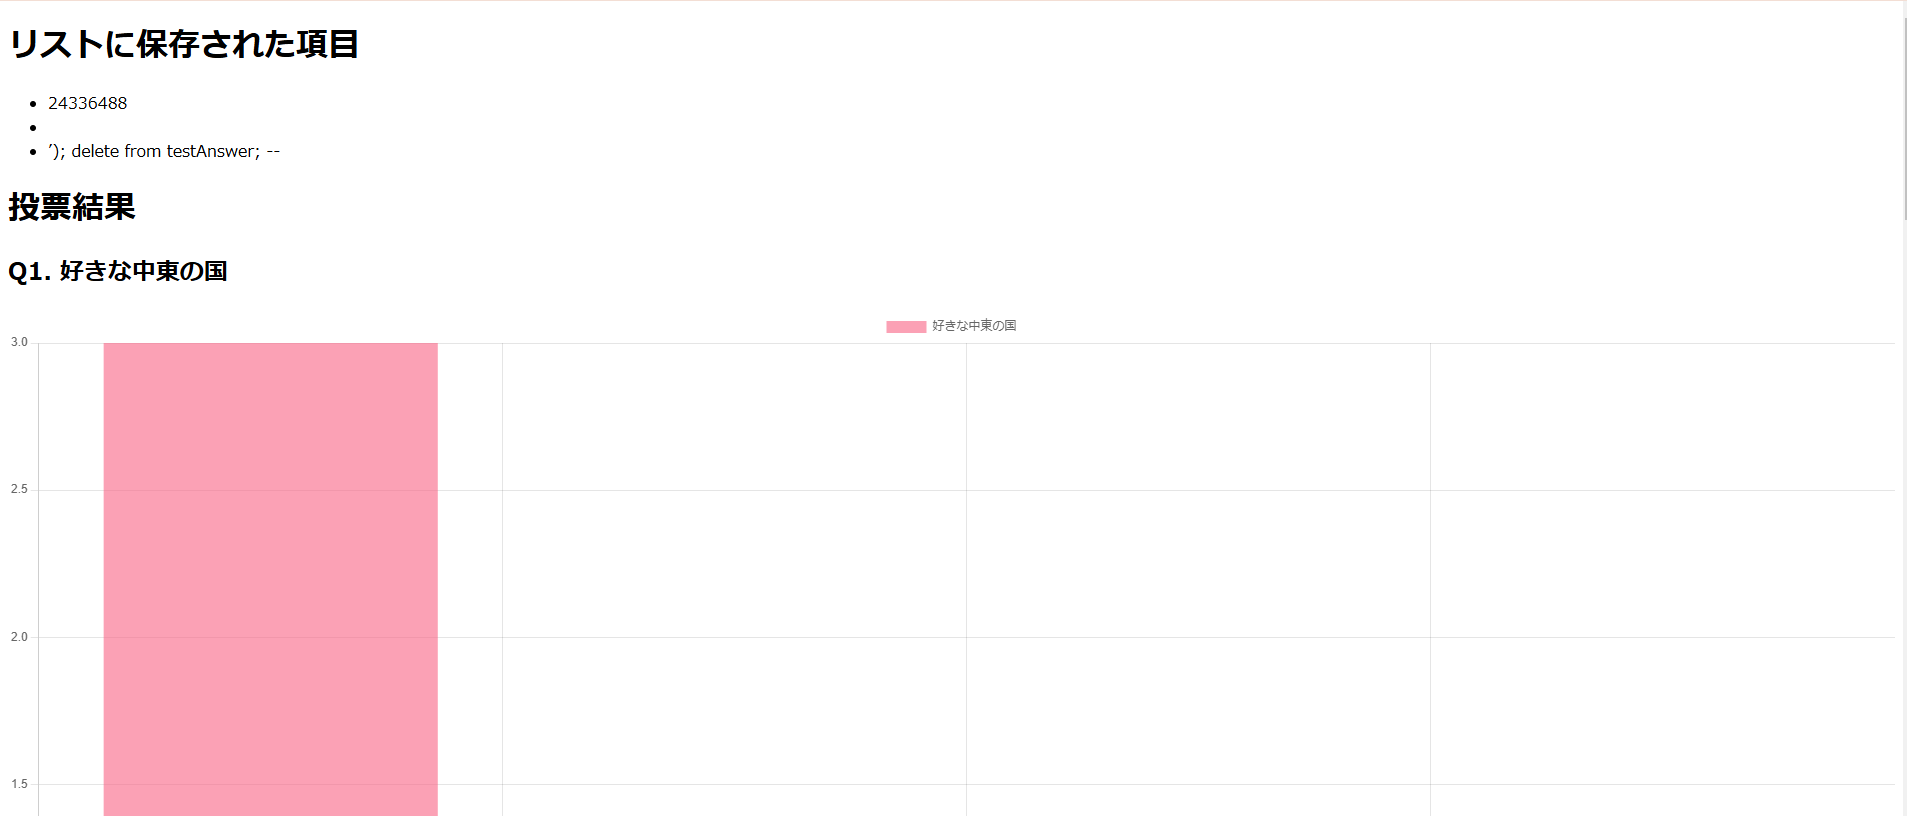
\includegraphics[width=\textwidth]{img/security/after_1.png}
    \subcaption{結果画面}
  \end{minipage}
  \caption{'); delete from testAnswer; --を入力した際の様子}
  \label{SQL_Injection1}
\end{figure}

\begin{figure}[H]
  \centering
  % 左側の画像
  \begin{minipage}[t]{0.45\textwidth}
    \centering
    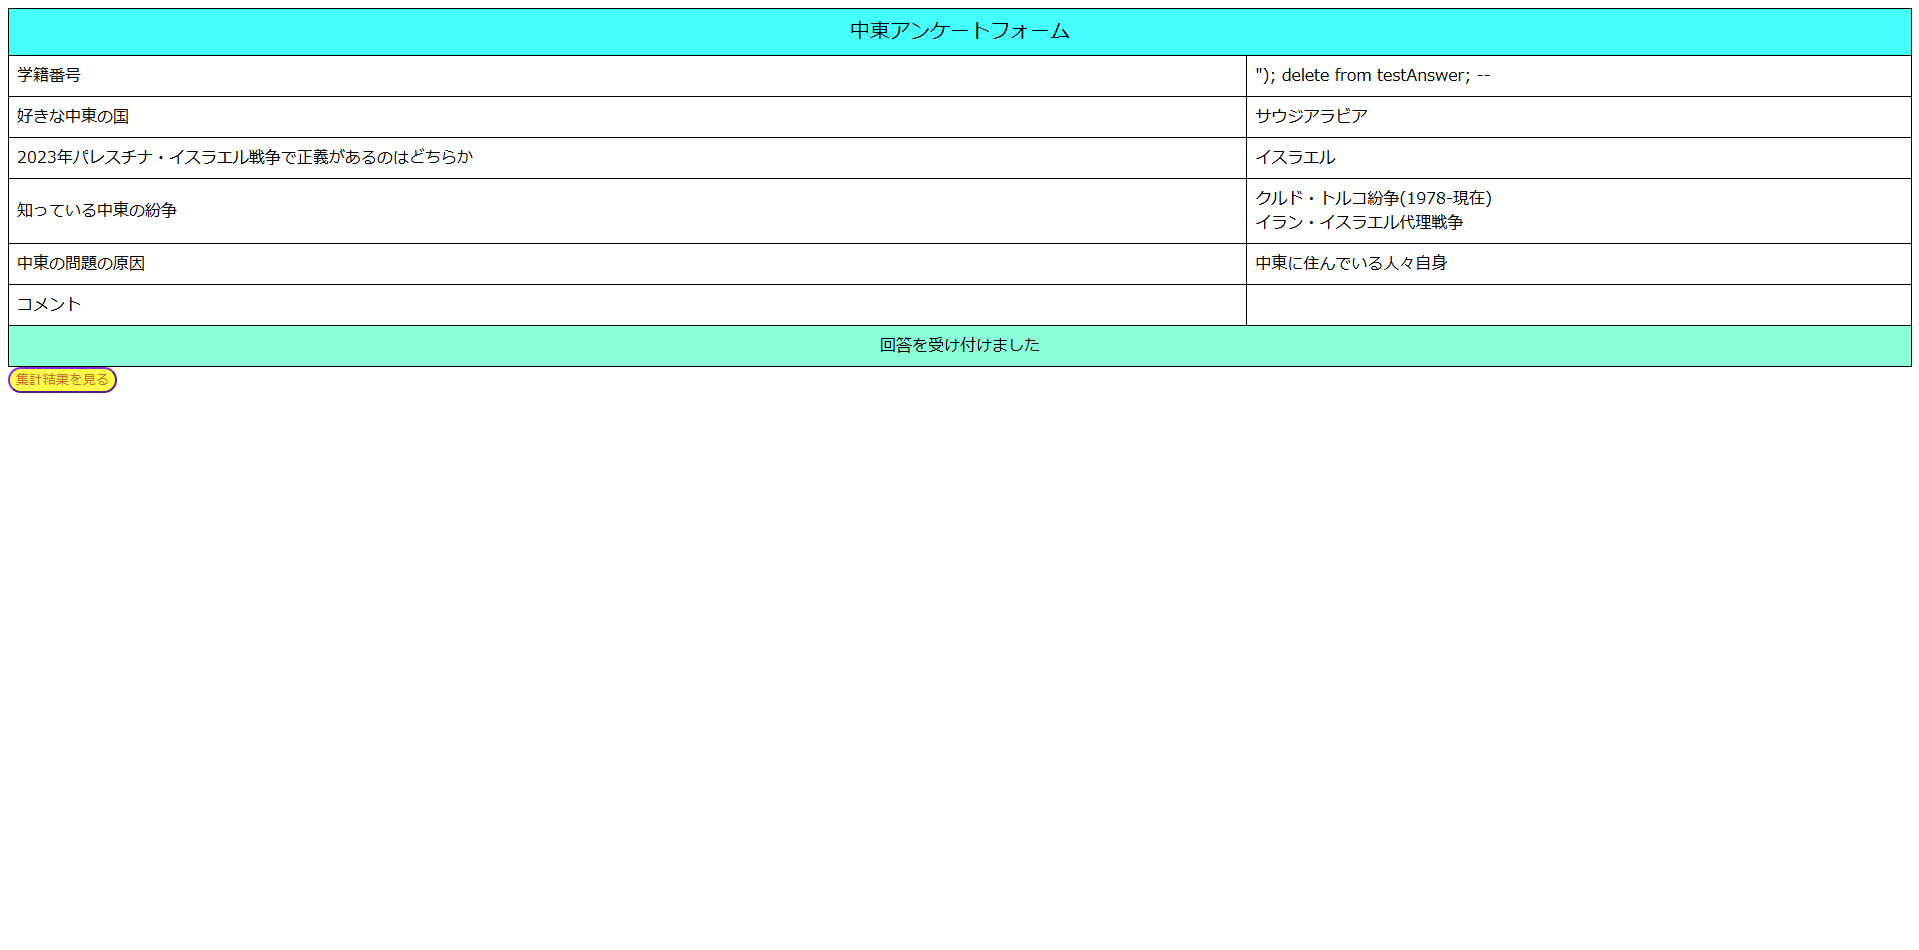
\includegraphics[width=\textwidth]{img/security/before_2.png}
    \subcaption{入力画面}
  \end{minipage}
  \hfill % 隙間を作る
  % 右側の画像
  \begin{minipage}[t]{0.45\textwidth}
    \centering
    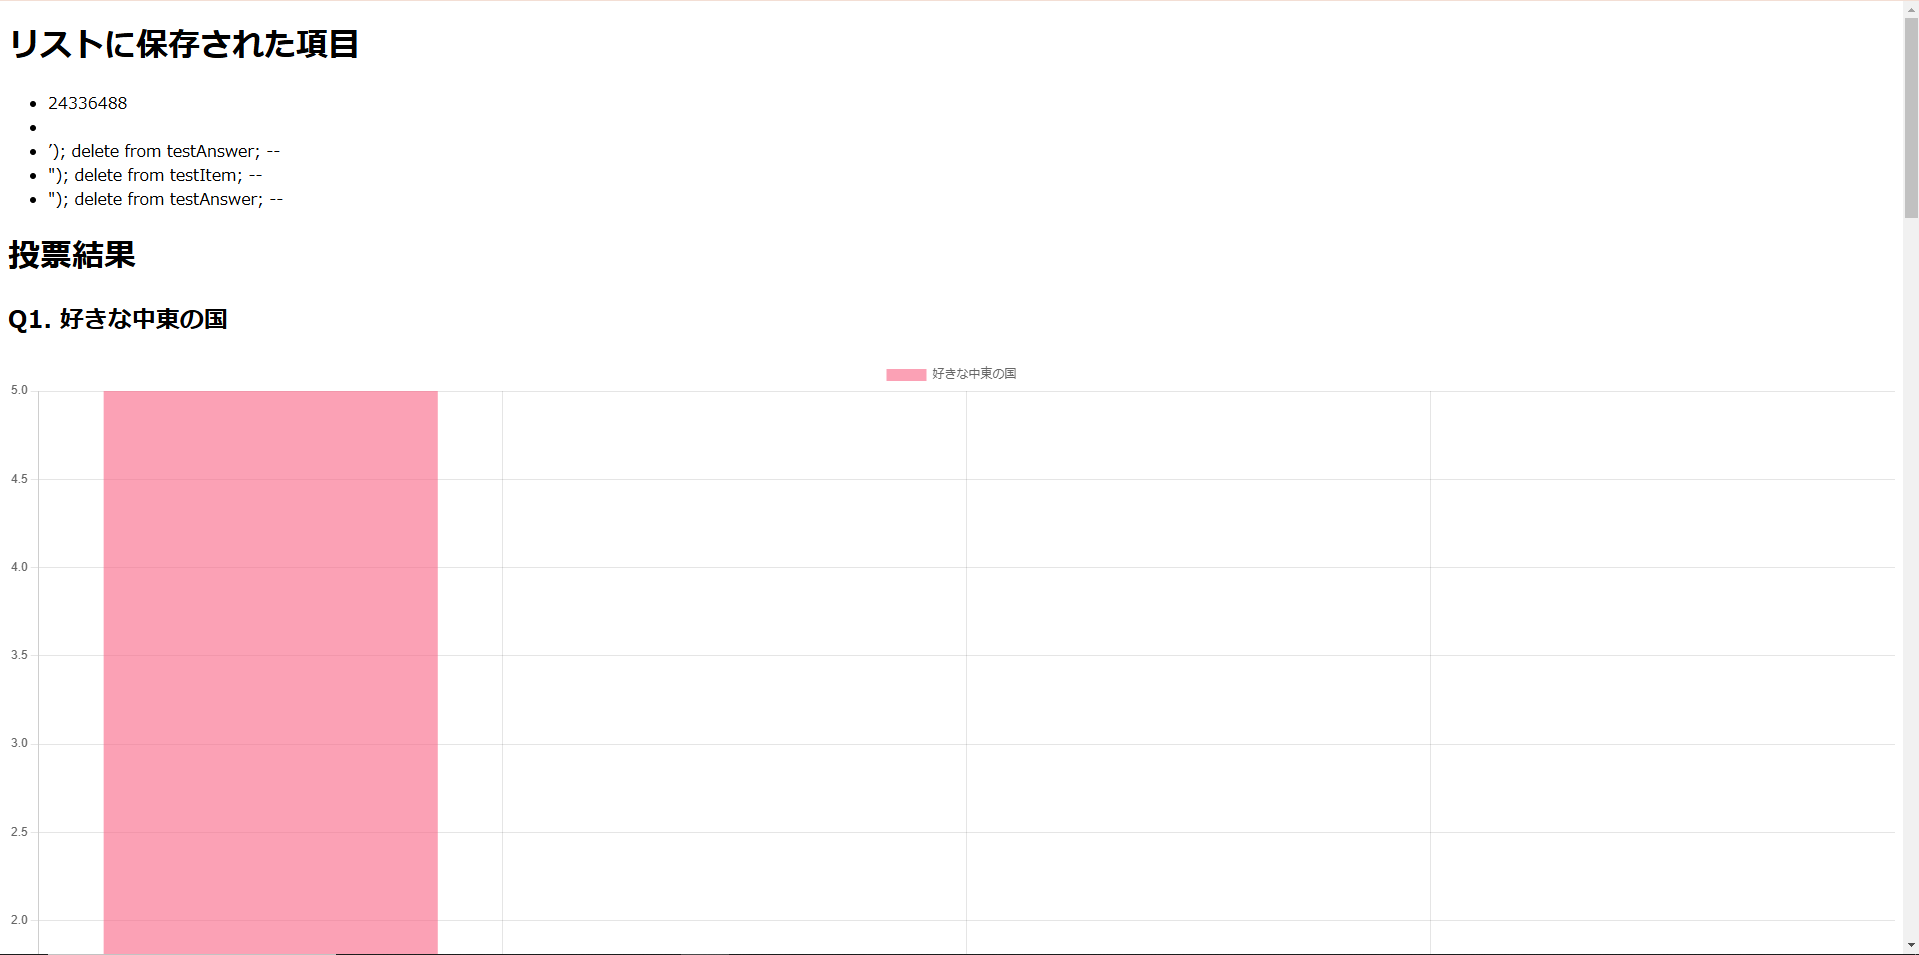
\includegraphics[width=\textwidth]{img/security/after_2.png}
    \subcaption{結果画面}
  \end{minipage}
  \caption{"); delete from testAnswer; --を入力した際の様子}
  \label{SQL_Injection2}
\end{figure}

これらの入力を行った後データベースを確認したが,データの欠損などは確認できなかった.
また,入力した値がそのまま出力画面に表示されていることが確認できる.

この結果から,変換等が行われ,全く同じ形で送信されていない可能性を考え作成したAPIから送られてきたJSONファイルの中身を確認した.
JSONファイルをソースコード\ref{answer}に示す.
\begin{lstlisting}[caption=Answer.json,label=answer]
  [
    {
      "rid": 1037,
      "studentId": "24336488",
      "country0": 1,
      "country1": 0,
      "country2": 0,
      "country3": 0,
      "isJustice": 0,
      "know0": 1,
      "know1": 1,
      "know2": 0,
      "know3": 0,
      "problem0": 1,
      "problem1": 0,
      "problem2": 0,
      "problem3": 0,
      "problem4": 0
    },
    {
      "rid": 1038,
      "studentId": "\u003Cscript\u003Ealert(document.cookie);\u003C/script\u003E",
      "country0": 1,
      "country1": 0,
      "country2": 0,
      "country3": 0,
      "isJustice": 0,
      "know0": 1,
      "know1": 0,
      "know2": 1,
      "know3": 0,
      "problem0": 1,
      "problem1": 0,
      "problem2": 0,
      "problem3": 0,
      "problem4": 0
    },
    {
      "rid": 1039,
      "studentId": "'); delete from testAnswer; --",
      "country0": 1,
      "country1": 0,
      "country2": 0,
      "country3": 0,
      "isJustice": 1,
      "know0": 1,
      "know1": 1,
      "know2": 0,
      "know3": 0,
      "problem0": 1,
      "problem1": 0,
      "problem2": 0,
      "problem3": 0,
      "problem4": 0
    },
    {
      "rid": 1040,
      "studentId": "\"); delete from testItem; --",
      "country0": 1,
      "country1": 0,
      "country2": 0,
      "country3": 0,
      "isJustice": 0,
      "know0": 1,
      "know1": 1,
      "know2": 0,
      "know3": 0,
      "problem0": 1,
      "problem1": 0,
      "problem2": 0,
      "problem3": 0,
      "problem4": 0
    },
    {
      "rid": 1041,
      "studentId": "\"); delete from testAnswer; --",
      "country0": 1,
      "country1": 0,
      "country2": 0,
      "country3": 0,
      "isJustice": 0,
      "know0": 1,
      "know1": 1,
      "know2": 0,
      "know3": 0,
      "problem0": 1,
      "problem1": 0,
      "problem2": 0,
      "problem3": 0,
      "problem4": 0
    },
    {
      "rid": 1042,
      "studentId": "\\\"); delete from testAnswer; --\"",
      "country0": 1,
      "country1": 0,
      "country2": 0,
      "country3": 0,
      "isJustice": 0,
      "know0": 1,
      "know1": 1,
      "know2": 0,
      "know3": 0,
      "problem0": 1,
      "problem1": 0,
      "problem2": 0,
      "problem3": 0,
      "problem4": 0
    },
    {
      "rid": 1043,
      "studentId": "\\\"); delete from testAnswer; --\"",
      "country0": 1,
      "country1": 0,
      "country2": 0,
      "country3": 0,
      "isJustice": 0,
      "know0": 1,
      "know1": 1,
      "know2": 0,
      "know3": 0,
      "problem0": 1,
      "problem1": 0,
      "problem2": 0,
      "problem3": 0,
      "problem4": 0
    }
  ]  
\end{lstlisting}
これを見るとわかるように,バックスラッシュやダブルクォーテーションのようなメタ文字がただの文字として出力できるように変更されている.
おそらくこれにより不正なSQL文送られ,正しくデータベースが破壊されなかったと考えられる.

ここで,変換の際にでるバックスラッシュをどうにかしてコマンドではなく文字として出力できれば上手くデータベースを破壊できるのではないかと考え,
\textbf{\textbackslash "); delete from testAnswer; --}と入力した.
その結果を図\ref{back}に示す.
\begin{figure}[H]
  \centering
  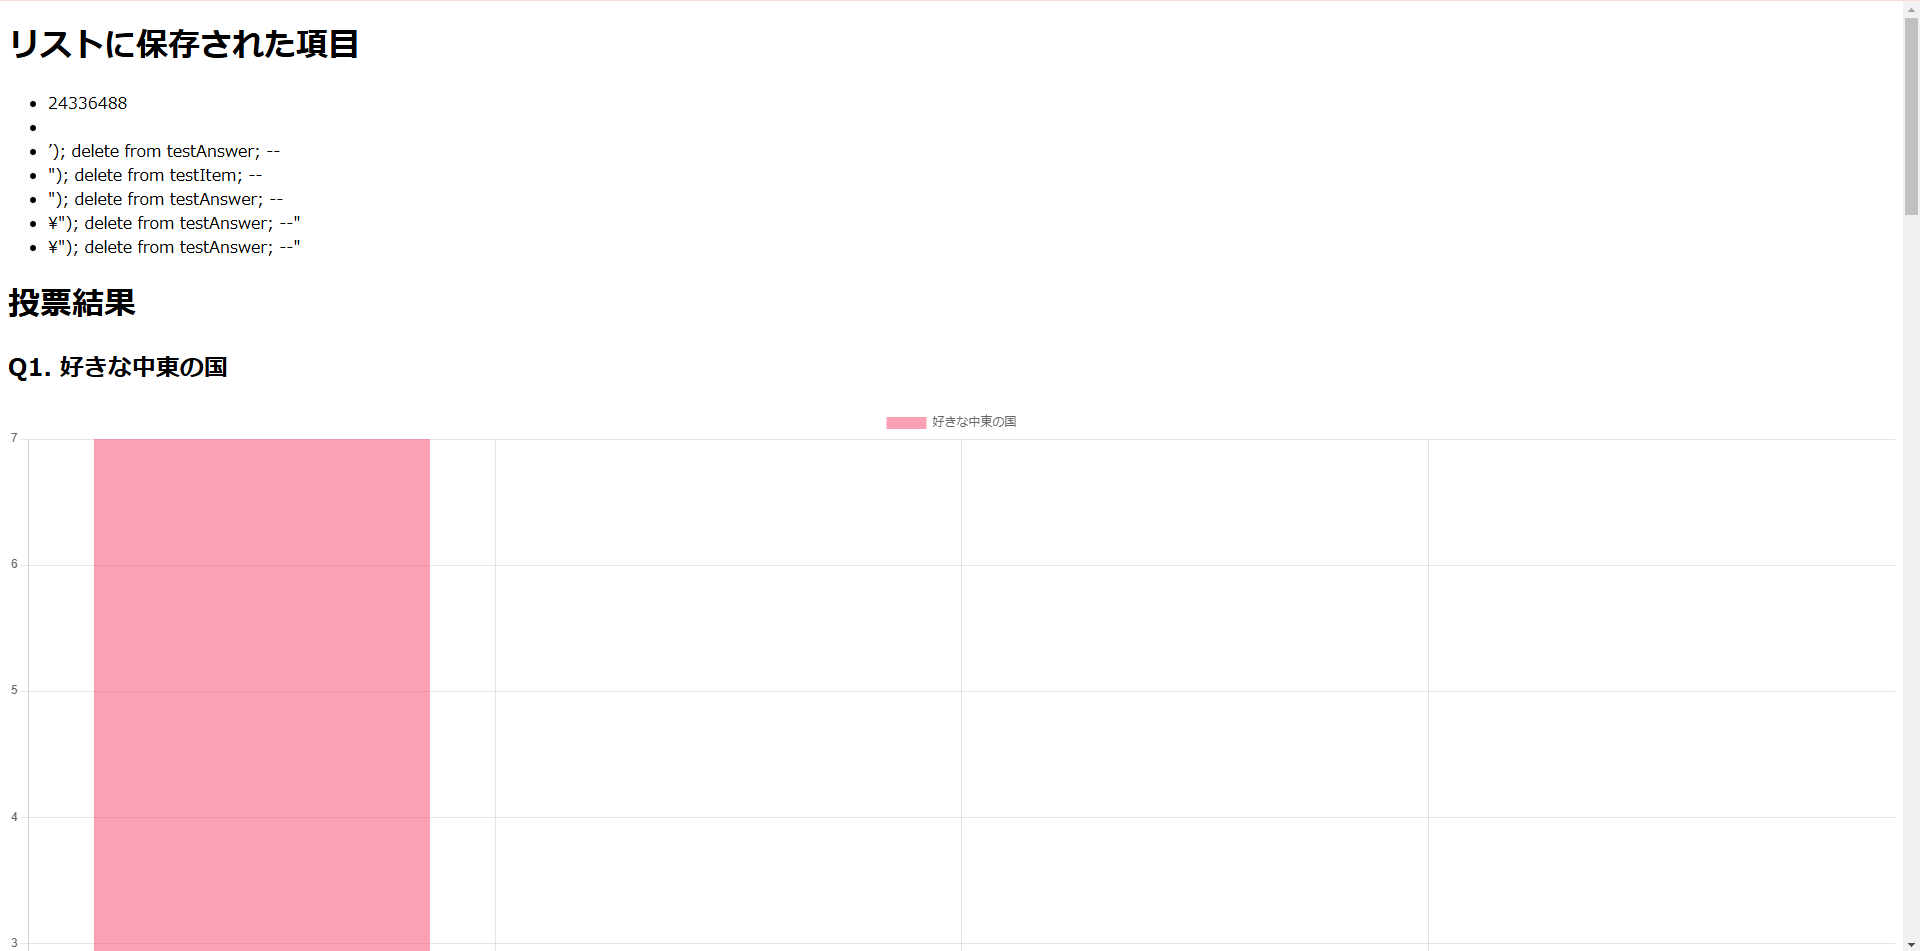
\includegraphics[width=0.8\textwidth]{img/security/back.png}
  \caption{\textbackslash "); delete from testAnswer; --と入力した際の様子}
  \label{back}
\end{figure}
もちろん上手くいかなかった.
ソースコード\ref{answer}のrid:1042がこの入力と同じものなのだが,
これも図\ref{SQL_Injection2}の場合と同様にメタ文字がただの文字として出力できるように変更されているためであると考えられる.

\subsubsection{クロスサイトスクリプティング}\label{xss}
クロスサイトスクリプティングとは,ユーザー入力に悪意のあるスクリプトを埋め込み,他のユーザーのブラウザでそのスクリプトを実行させる攻撃のことである.
今回はGoogle Choromeにて\textbf{\textless script\textgreater window.location='https://www.yahoo.co.jp/';\textless /script\textgreater}と入力して攻撃を試みた.
入力して送信ボタンを押した際の結果をそれぞれ図\ref{script}に示す.

\begin{figure}[tb]
  \centering
  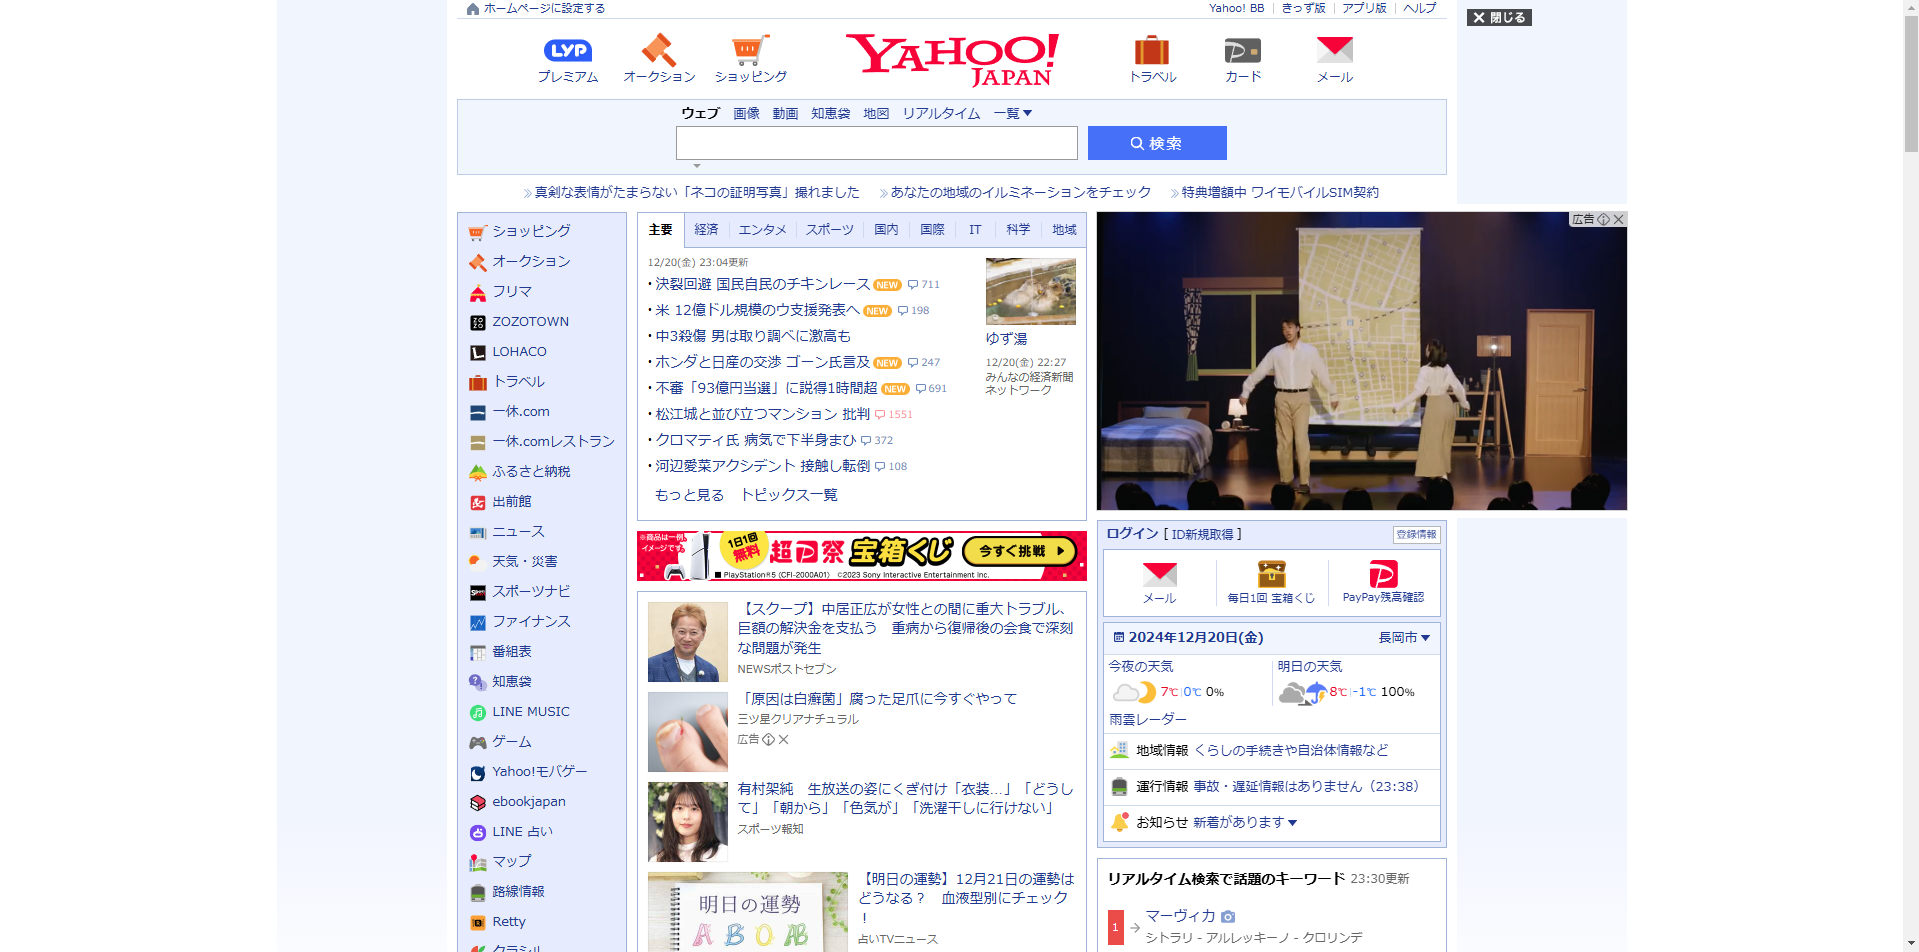
\includegraphics[width=0.8\textwidth]{img/security/yahoo.png}
  \caption{入力した際の結果}
  \label{script}
\end{figure}

画像を見れば分かる通り\url{https://www.yahoo.co.jp/}に遷移した.
Webサイトで入力をした際はデータベースに保存される前に遷移したため,ResultServlet.jspなどでこのページに遷移することはなかった.
また,図\ref{app_yahoo}のようにスマートフォンアプリで入力した際はデータ自体がデータベースへ送られることはなかった.
\begin{figure}[H]
  \centering
  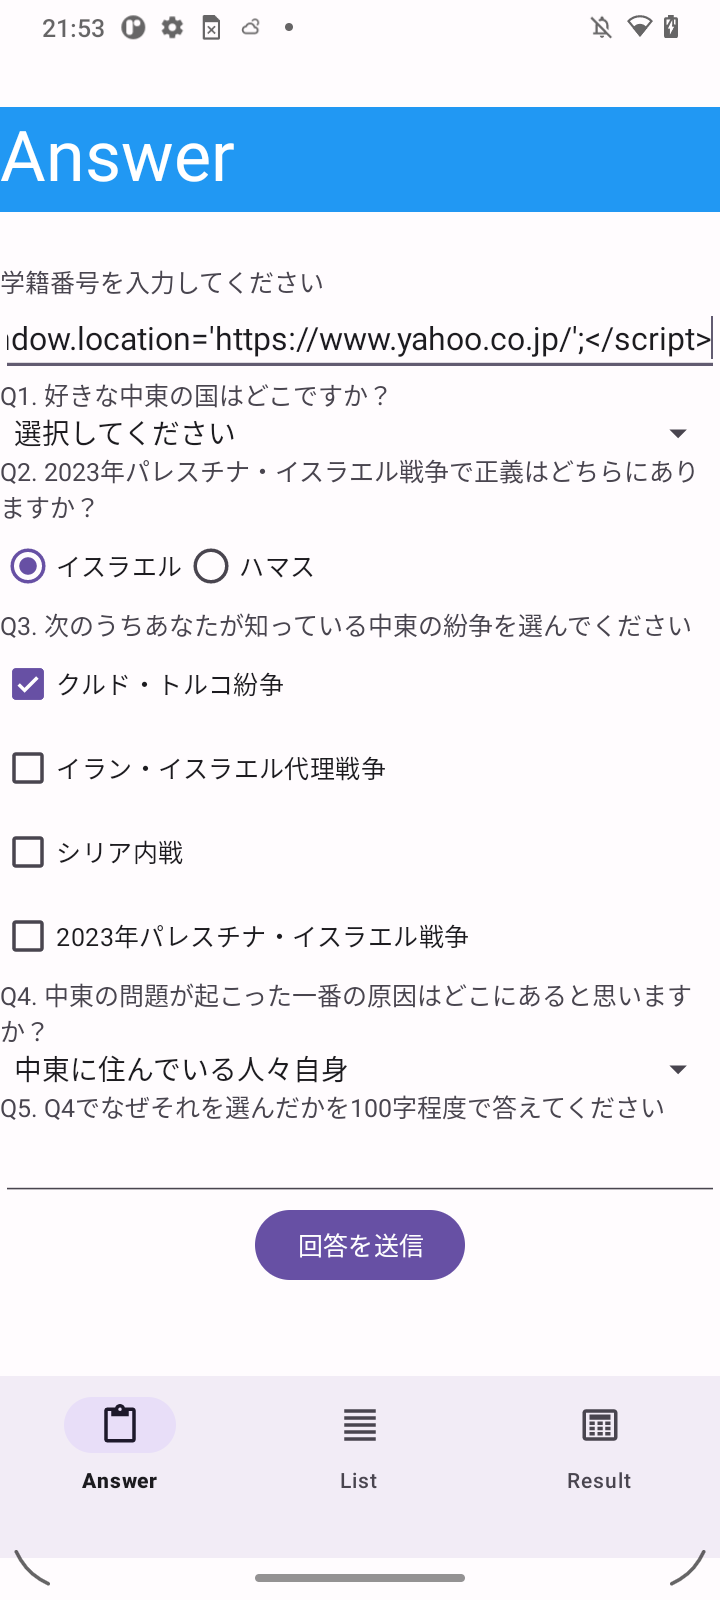
\includegraphics[width=0.4\textwidth]{img/security/app_yahoo.png}
  \caption{スマートフォンアプリからXSSを試みた様子}
  \label{app_yahoo}
\end{figure}
これらのことからわかるように,Webサイトにスクリプトを埋め込むことは可能なので,悪意のあるサイトへの誘導やWebアプリを壊しかねないスクリプトの入力などが考えられる.
そのため,メタ文字を入力不可にするなどして対策するべきである.
\subsubsection{セッションハイジャック}
セッションハイジャックとは,\ref{xss}節と同様に,Google Choromeで\\\textbf{\textless script\textgreater alert(document.cookie);\textless /script\textgreater}と入力して攻撃を試みた.
Q1.jspやResultServlet.jspのような,この文字列が表示され得る場所で出てきたアラートを図\ref{alert}に示す.
\begin{figure}[H]
  \centering
  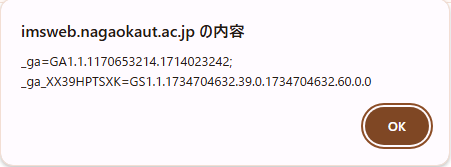
\includegraphics[width=0.8\textwidth]{img/security/alert.png}
  \caption{クロスサイトスクリプティングをした際の出力画面}
  \label{alert}
\end{figure}

\_gaや\_ga\_XX39HPTSXKはGoogle Analyticsが利用するCookieであり,これらのCookieは匿名化されたデータを使用しているため,個人情報(名前,住所など)は含まれていない.
しかし,ここに表示されているIPアドレスはトラッキングに利用される可能性があるため防ぐことが好ましい.
また,このアラートは,out.println()などを用いて表示されるすべての場所で出現したため,\ref{xss}節と同様に,悪意のあるサイトへの誘導やWebアプリを壊しかねないスクリプトを入力されてしまう可能性がある.
\section{感想}
%  ※ここは採点の対象外です。
%   今回の演習の内容について感想などあれば記述して下さい。
%  次年度以降の演習の実施に役立てたいと思います。
\begin{itemize}
  \item for QandAと書いてあるのに中身がほぼItemManagerなのをやめてほしい.
        そもそも配らないか,しっかり中身を書き換えたものにしてほしい.
        それか,書き換える部分はスライドに残すなどしてほしい.
  \item
\end{itemize}

% 参考文献
\begin{thebibliography}{99}
  \bibitem{qiita}MVC、3層アーキテクチャから設計を学び始めるための基礎知識 \#初心者 - Qiita\\\url{https://qiita.com/os1ma/items/7a229585ebdd8b7d86c2}
\end{thebibliography}

\end{document}